\documentclass[12pt]{article}
\usepackage{parskip}
\usepackage{amsmath}
\usepackage{pdfpages}
\usepackage[margin=.6in]{geometry}
\begin{document}
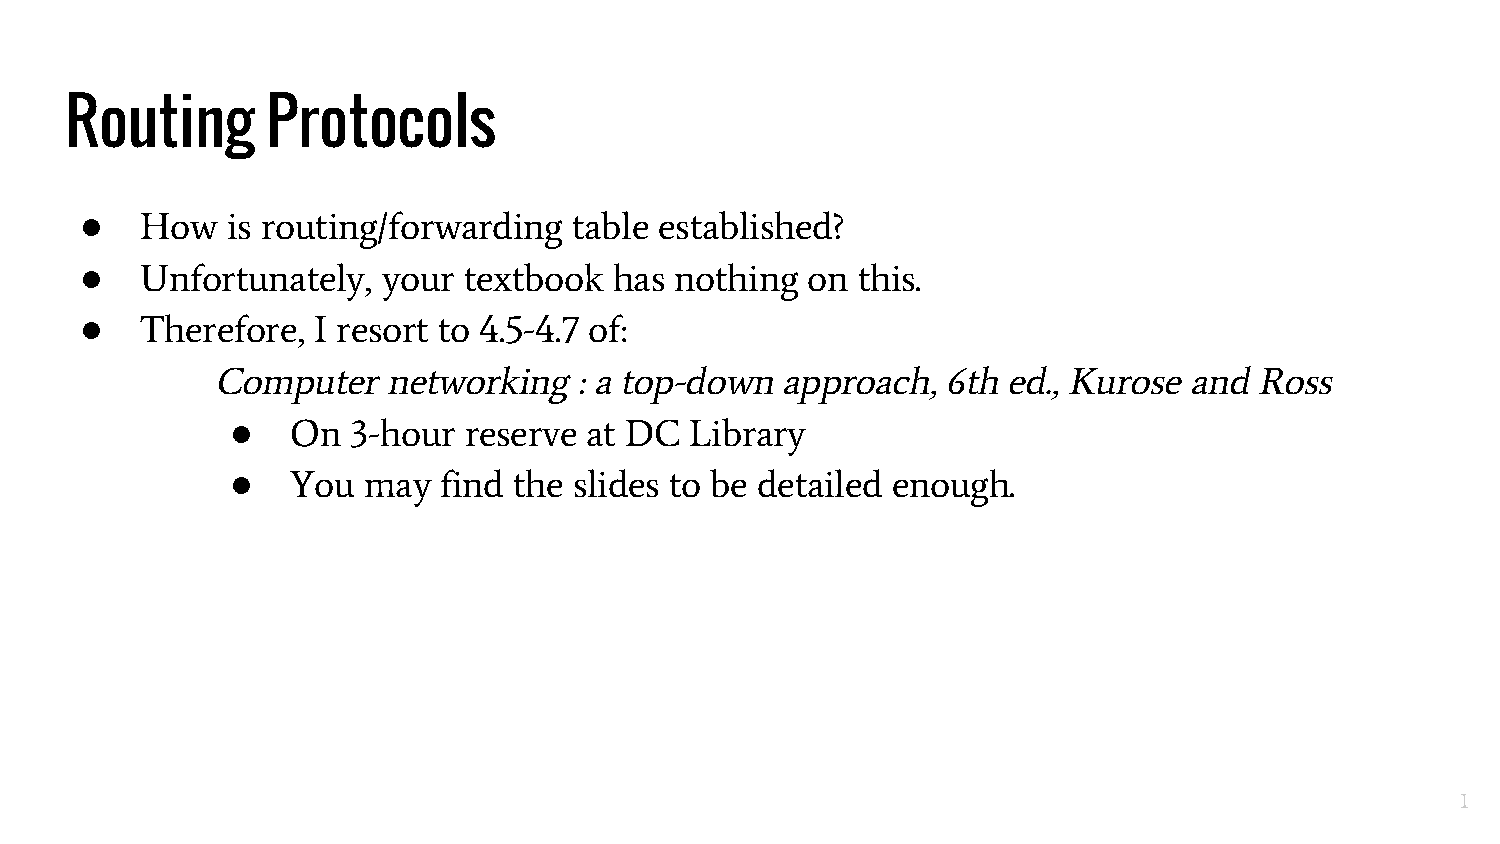
\includepdf[pages=1]{slides}
Often manual configuration of routs is not practical (they can be super complicated and dynamic). Thus we get routing protocols. There is nothing in the current textbook for this so you need to look at the older textbook.

\includepdf[pages=4]{slides}
The whole point of a routing protocol is to figure out what the fowarding table should look like. Basically where the packets should go next.

\includepdf[pages=5]{slides}
\includepdf[pages=6]{slides}
We abstract this out to a graph. We have nodes and weighted edges (often the nodes are routers or devices). Often the cost is multidimensional which can make things complicated. We want to try to find the cheapest path through this graph. 

\includepdf[pages=7]{slides}
\includepdf[pages=9-17]{slides}
Djikstra's algorithm shit. 

\includepdf[pages=18-25]{slides}
We can keep track of distance vector tables that say the total cost of the path to another node and the next hop in the path. These values are caluclated using djikstra's algorithm. You keep updating it by adding and taking mins as you go. Basically nodes keep each other in sync by sending their distance tables to each other and if a better path occurs updating to match it. 

When the distance between two nodes updates shit gets a bit crazy. Basically the nodes that notices the change will update its table to reflect it. If the path is now shorter it moves very quickly sending it around. If the path increases it moves incredibly slowly. We can get loops because the tables don't all update at the same time so one table can think that one way is the optimal math while a table with fresher data knows that another path is optimal. This results in data moving around a ton.

\textbf{Counting to infinity} Say Y notices the update first. It sees that to get to X costs 60 so it looks for a faster route. Z says that it can get to X with a cost of 5 so Y wants to use Z. Once this is done Y broadcasts its change and Z decides to update. Then Z updates its self. It does the same logic where it sees that Y can reach X with a cost of six so it wants to go through there. Then Z broadcasts it change. This goes back and forth for a while until it gets its shit together.

\textbf{poisoned reverse}: with this Z advertises to Y that is has a cost of infinity to get anywhere. This makes Y go directly to X and broadcasts the update to Z. This puts an infinity to get to Z. Now Z has to update itself. It updates its routing table to now use the direct connects to X and Y (because these are the cheapest known paths). This is how we get around the counting to infinity problem. Poisoned reverse is not always sufficient. He gives a good example for this, see supplementary notes on it. There is going to be a question about this on the exam


\includepdf[pages=26]{slides}
LOOK THIS UP IN THE TEXTBOOK


\includepdf[pages=29]{slides}
Every system figures out which routing protocol works for them so a gateway router is needed to talk between them. This allows us to categoritze routers by the routing protocol that they follow.

\includepdf[pages=30]{slides}
Theres a intra routing algorithm and inter and these could be different and are categorized by AS. 

\includepdf[pages=31-32]{slides}
Subnet X is reachable by AS3 and not AS2, then the interAS protocol propogates that information to all interal routers. We use intraAS to see that  1Bs least cost to 1C is through some interface so it makes a entry for that.

\includepdf[pages=33]{slides}
If we now know that X is reachable by AS1, we now have a choice for 1d to figure out the least cost path to get a packet through to X. This is much harder to figure out and done through interAS. 

\includepdf[pages=34]{slides}


\includepdf[pages=36]{slides}
\includepdf[pages=37]{slides}
Interesting to note that we count a hope from an internal port to external (so the hop to u is one).

\includepdf[pages=39]{slides}
In this example if we wanted to have the route from internal to external to be 0 we would have the distance from D to W to be equal to 0 which is clearly not true. This is why we make that cost equal to 1.

\includepdf[pages=40]{slides}
If we haven't heard an advertisement in a while we will deem the node dead. Usually the time span is about 3 minutes. 

\includepdf[pages=41-76]{slides}






\end{document}